%%
% This is an Overleaf template for presentations
% using the TUM Corporate Desing https://www.tum.de/cd
%
% For further details on how to use the template, take a look at our
% GitLab repository and browse through our test documents
% https://gitlab.lrz.de/latex4ei/tum-templates.
%
% The tumbeamer class is based on the beamer class.
% If you need further customization please consult the beamer class guide
% https://ctan.org/pkg/beamer.
% Additional class options are passed down to the base class.
%
% If you encounter any bugs or undesired behaviour, please raise an issue
% in our GitLab repository
% https://gitlab.lrz.de/latex4ei/tum-templates/issues
% and provide a description and minimal working example of your problem.
%%

\PassOptionsToClass{onlytextwidth}{beamer}

\documentclass[
  german,            % define the document language (english, german)
  aspectratio=169,    % define the aspect ratio (169, 43)
  % handout=2on1,       % create handout with multiple slides (2on1, 4on1)
  % partpage=false,     % insert page at beginning of parts (true, false)
  % sectionpage=true,   % insert page at beginning of sections (true, false)
]{tumbeamer}


% load additional packages
\usepackage{tikz}
\usepackage{circuitikz}
\usepackage{url}
\usepackage{hyperref}
\usepackage{pgf}
\usepackage{pgfplots}
\usepackage{babel}[ngerman]
\usepackage{csquotes}[autostyle]
\usepackage[useregional]{datetime2}
\usepackage{float}
\usepackage{graphicx}
\usepackage{amsmath}
\usepackage{xcolor}
\usepackage[cache=true]{minted}
\usemintedstyle{borland}
\usepackage{listings}
\usepackage{tikz-timing}
\usepackage{tabularx}


% tikz  
\usetikzlibrary{fit, matrix, calc, arrows, arrows.meta, positioning, patterns, patterns.meta, overlay-beamer-styles, riscvproc}

% processor
\definecolor{modblue}{HTML}{288DCC}
\ctikzset{processor/font=\fontfamily{lmss}\selectfont}

% https://tex.stackexchange.com/a/7045
\newcommand*\circled[1]{\tikz[baseline=(char.base)]{
		\node[shape=circle,draw,inner sep=2pt, font=\scriptsize] (char) {#1};}}

\newcommand*\colorcirc[1]{\tikz[baseline=(char.base)]{
		\node[shape=circle,fill=#1,inner sep=2pt] {};}}

\newcommand\n[1]{\mkern1mu\overline{\mkern-1mu#1}}

% requires circuitikz >= 1.1.0
% for distros with older distributions, install TeX Live manually
% instead of using your package manager
% see: https://tug.org/texlive/quickinstall.html
\ctikzset{logic ports=ieee}

% minted
\setminted{
	fontsize=\small, 
	frame=none,
	breaklines=true,
}

\captionsetup{labelformat=empty}

% image path
\graphicspath{ {./resources/}, {../riscv-circuitikz/figures/} }

% beamer
\setbeamercolor{footnote}{fg=black}
\setbeamercolor{footnote mark}{fg=black}
\renewcommand{\thempfootnote}{\arabic{mpfootnote}}

% presentation metadata
\title{Übung 08: Maschinensprache \\und Single-Cycle-Prozessor}
\subtitle{Einführung in die Rechnerarchitektur}
\author{Niklas Ladurner}

\institute{\theChairName\\\theDepartmentName\\\theUniversityName}
\date{\DTMdisplaydate{2025}{12}{05}{-1}}

\footline{\insertauthor~|~\insertshorttitle~|~\insertshortdate}


% macro to configure the style of the presentation
\TUMbeamersetup{
  title page = TUM tower,         % style of the title page
  part page = TUM toc,            % style of part pages
  section page = TUM toc,         % style of section pages
  content page = TUM more space,  % style of normal content pages
  tower scale = 1.0,              % scaling factor of TUM tower (if used)
  headline = TUM threeliner,      % which variation of headline to use
  footline = TUM default,         % which variation of footline to use
  % configure on which pages headlines and footlines should be printed
  headline on = {title page},
  footline on = {every page, title page=false},
}

\begin{document}

\maketitle

\begin{frame}[c]{Feedback}{}
	\begin{columns}[c]
		\begin{column}{0.5\textwidth}
			\begin{center}
				\LARGE  \href{https://t1p.de/era2526}{t1p.de/era2526}\\
				
\includegraphics[height=0.5\textheight]{feedback_qr.pdf}
			\end{center}
		\end{column}
		\begin{column}{0.5\textwidth}
			\begin{center}
				\LARGE  \href{https://home.in.tum.de/~ladu/}{home.in.tum.de/\string~ladu/}\\
				\includegraphics[height=0.5\textheight]{website_qr.pdf}
			\end{center}
		\end{column}
	\end{columns}
\end{frame}

\begin{frame}[c, fragile]{}{}
	\begin{center}
		\LARGE  Keine Garantie für die Richtigkeit der Tutorfolien.

		\Large Bei Unklarheiten/Unstimmigkeiten haben VL/ZÜ-Folien recht!
	\end{center}
\end{frame}

\begin{frame}[c, fragile]{Instruktionstypen\footnote{NB: Die Befehle für die einzelnen Typen sind nur auszugsweise angegeben.}}{}
	\setlength{\extrarowheight}{5pt}
	\begin{tabularx}{0.9\textwidth}{lXl}
		\texttt{R}  & Register-Register-Operationen                      & \texttt{add}, \texttt{sub}, \texttt{sll}  \\
		\texttt{I}  & Short Immediates (12 Bit) und Ladebefehle          & \texttt{jalr}, \texttt{lw}, \texttt{ori}  \\
		\texttt{S}  & Speicherbefehle                                    & \texttt{sw}, \texttt{sh}                  \\
		\texttt{B}  & Branches (bedingte Sprünge)                        & \texttt{beq}, \texttt{blt}, \texttt{bgtu} \\
		\texttt{U}  & Long Immediates (20 Bit)                           & \texttt{lui}, \texttt{auipc}              \\
		\texttt{J}  & Jumps (unbedingte Sprüge) mit Long Immediate       & \texttt{jal}                              \\
		\texttt{R4} & Floating-Point-Operationen, für ERA nicht relevant &                                           \\
	\end{tabularx}
\end{frame}

\begin{frame}[c, fragile]{Assemblierung}{}
	\begin{center}
		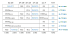
\includegraphics[width=0.75\textwidth]{w08_risc_v_types.pdf}\\
		\vspace*{\baselineskip}
		\tiny (Quelle: Vorlesungsmaterialien ERA)
	\end{center}

\end{frame}

\begin{frame}[c, fragile]{Assemblierung: Beispiel}{}
	\begin{columns}[c]
		\begin{column}{0.5\textwidth}
			\begin{enumerate}
				\item<1-> Instruktionstyp feststellen \only<2->{$\rightarrow$ \texttt{R}}
				\item<2-> Dazugehöriges Layout in Tabelle finden
				\item<3-> Instruktion in Tabelle finden
				\item<4-> Instruktionsspezifische Werte ablesen
				\item<5-> Registermapping: ($\texttt{zero} \mapsto \texttt{x0}, \ldots, \texttt{t6} \mapsto \texttt{x31}$)
				\item<6-> Binärzahl zusammenbauen
			\end{enumerate}
		\end{column}%
		\begin{column}{0.5\textwidth}
			\centering
			\begin{tikzpicture}
				\def\spc{0.5cm}
				\node[draw=none] (instr) at (0,0)  {\large\texttt{xor t2, t1, t0}};

				\node[below=\spc of instr, visible on=<2->] (tabtype) {
					
\includegraphics[width=\textwidth]{w08_r_type.pdf}
				};

				\node[below=\spc of tabtype, visible on=<3->] (tabinstr)  {
					\resizebox{\textwidth}{!}{
						\setlength{\extrarowheight}{2.5pt}
						\begin{tabular}{|l|c|c|c|l|}
							\hline
							\rowcolor[HTML]{0078C3}
							{\color{white}\textbf{op}} & {\color{white}\textbf{funct3}} & {\color{white}\textbf{funct7}} & {\color{white}\textbf{Type}} & {\color{white}\textbf{Instruction}} \\ \hline
							0110011 (51)               & 100                            & 0000000                        & R                            & \texttt{xor rd, rs1, rs2}           \\ \hline
						\end{tabular}
					}
				};
			
			\node[draw=none, below=\spc of tabinstr, visible on=<5->] (regmap) {\large\texttt{t2} $\mapsto$ \texttt{x7}, \texttt{t1} $\mapsto$ \texttt{x6}, \texttt{t0} $\mapsto$ \texttt{x5} };
			\end{tikzpicture}
		\end{column}
	\end{columns}
\begin{center}
	\vspace*{0.5cm}
	\begin{center}
		\Large
%		$(0000000\;00101\;00110\;100\;00111\;0110011)_2 = \textrm{0x005343B3}$
		\only<6>{\texttt{funct7}\quad\texttt{rs2}\quad\texttt{rs1}\quad\texttt{funct3}\quad\texttt{rd}\quad\texttt{op}}
		\only<7>{\textcolor{TUMBlue}{\texttt{funct7}}\quad\texttt{rs2}\quad\texttt{rs1}\quad\textcolor{TUMBlue}{\texttt{funct3}}\quad\texttt{rd}\quad\textcolor{TUMBlue}{\texttt{op}}}
		\only<8>{\textcolor{TUMBlue}{\texttt{0000000}}\quad\texttt{rs2}\quad\texttt{rs1}\quad\textcolor{TUMBlue}{\texttt{100}}\quad\texttt{rd}\quad\textcolor{TUMBlue}{\texttt{0110011}}}
		\only<9>{\texttt{0000000}\quad\texttt{rs2}\quad\texttt{rs1}\quad\texttt{100}\quad\texttt{rd}\quad\texttt{0110011}}
		\only<10>{\texttt{0000000}\quad\textcolor{TUMBlue}{\texttt{rs2}}\quad\textcolor{TUMBlue}{\texttt{rs1}}\quad\texttt{100}\quad\textcolor{TUMBlue}{\texttt{rd}}\quad\texttt{0110011}}
		\only<11>{\texttt{0000000}\quad\textcolor{TUMBlue}{\texttt{00101}}\quad\textcolor{TUMBlue}{\texttt{00110}}\quad\texttt{100}\quad\textcolor{TUMBlue}{\texttt{00111}}\quad\texttt{0110011}}
		\only<12>{\texttt{0000000}\quad\texttt{00101}\quad\texttt{00110}\quad\texttt{100}\quad\texttt{00111}\quad\texttt{0110011}}
		\only<13>{\texttt{0b\;0000\;0000\;0101\;0011\;0100\;0011\;1011\;0011 = 0x005343B3}}
	\end{center}
\end{center}
\end{frame}


\begin{frame}[c]{RISC-V Single-Cycle-Prozessor}{}
	\begin{center}
		\resizebox{0.75\textwidth}{!}{
			\input{riscv_sc_branchlogic.tikz}
		}
	\end{center}
\end{frame}

\begin{frame}[c, fragile]{}{}
	\begin{center}
		\LARGE Fragen?
	\end{center}
\end{frame}


\begin{frame}[c, fragile]{Links}{}
	\begin{itemize}
		\item Zulip: \href{https://zulip.in.tum.de/#narrow/channel/3255-ERA-Tutorium-.E2.80.93-Mi-1600-3}{\enquote{ERA Tutorium -- Mi-1600-3}}
		      bzw. \href{https://zulip.in.tum.de/#narrow/channel/3264-ERA-Tutorium-.E2.80.93-Fr-1500-1}{\enquote{ERA Tutorium -- Fr-1500-1}}
		\item \href{https://www.moodle.tum.de/course/view.php?id=111440}{ERA-Moodle-Kurs}
		\item \href{https://artemis.tum.de/courses/516}{ERA-Artemis-Kurs}
		\item \href{https://courses.edx.org/assets/courseware/v1/f06a2dc0c856f60ec0711e9f5e1c98cf/asset-v1:HarveyMuddX+ENGR85B+1T2023+type@asset+block/FinalReferences.pdf}{Prozessor-Assets (kein offizielles Material!)}
		\item \href{https://riscvasm.lucasteske.dev/}{RISC-V Assembler}
	\end{itemize}
\end{frame}

\maketitle

\end{document}
